\documentclass{article}
\usepackage{geometry}
\usepackage{graphicx}
\usepackage{amsmath}
\usepackage{algorithm}
\usepackage{algpseudocode}
\usepackage{dsfont}

\geometry{
a4paper,
right=20mm,
left=20mm,
top=10mm,
bottom=10mm,	
}

\begin{document}

\pagenumbering{gobble}

\begin{center}
\textbf{\huge CS772: Probabilistic Machine Learning} \\
\textbf{\huge Homework 3} \\
\vspace{5pt}
\textit{\Large Jayant Agrawal} \\
14282
\end{center}

\section*{Problem 1}
\textbf{Gibbs Sampling for Count Matrix Factorization} \\ \\
The generative model(likelihood and prior) given in the question is as follows:
$$X_{nm} \sim Poisson(u_n^Tv_m) \forall n,m $$
$$u_{nk} \sim Gamma(a_u, 1/b_u) \forall n,k $$
$$v_{mk} \sim Gamma(a_v, 1/b_v) \forall m,k $$
We can also write $ X_{nm} \sim Poisson(\sum_{k=1}^K u_{nk}v_{mk}) $. Using the first identity(given in the question), we can write it as:
$$ X_{nmk} \sim Poisson(u_{nk}v_{mk}) $$
We can now write posterior for $u_{nk}$ as follows:
$$p(u_{nk}|X,V,U_{-nk}) \propto \prod_{m=1}^M p(x_{nmk}|u_{nk},v_{mk})p(u_{nk})$$
$$ \propto \prod_{m=1}^M [\frac{exp(-u_{nk}v_{mk})(u_{nk}v_{mk})^{x_{nmk}}}{X_{nmk}}] [u_{nk}^{a_u-1}exp(-u_{nk}b_u)]$$
$$ \propto exp(-u_{nk}[b_u+\sum_{m=1}^Mv_{mk}])u_{nk}^{a_u+\sum_{m=1}^MX_{nmk}-1} $$
Since we know that poisson and gamma are conjugate, thus ignoring constants we can say that:
$$p(u_{nk}|X,V,U_{-nk}) \sim Gamma(a_u+\sum_{m=1}^MX_{nmk}, 1/(b_u+\sum_{m=1}^Mv_{mk}))$$
Similarly, the posterior of $v_{mk}$ is given by:
$$p(v_{mk}|X,V,V_{-mk}) \sim Gamma(a_v+\sum_{n=1}^NX_{nmk}, 1/(b_v+\sum_{n=1}^Nu_{nk}))$$
Using the second identity(given in question), we can get $X_{mnk}$ by sampling from multinoulli as :
$$[X_{nm1},..X_{nmK}]|X_{nm} \sim multinomial(X_{nm};[\frac{\eta_1}{\eta}, ..,\frac{\eta_K}{\eta} ])$$
where $\eta_k = u_{nk}v_{mk}$ and $\eta = \sum_{k=1}^K u_{nk}v_{mk} $
The Gibbs Sampling scheme can thus be given as:
\begin{itemize}
\item Sample $X_{nmk} \forall n,m,k$ using multinomial
\item Sample $u_{nk} \forall n,k$ from it's posterior
\item Sample $v_{mk} \forall m,k$ from it's posterior
\end{itemize}

These steps have to be done for each sample in an iterative fashion.

\section*{Problem 2}
\textbf{Implementing Gibbs Sampler for Count Matrix Factorization} \\ \\
\textit{Plots for MAE vs Iterations} \\ \\
\begin{figure}[h!]
\begin{center}
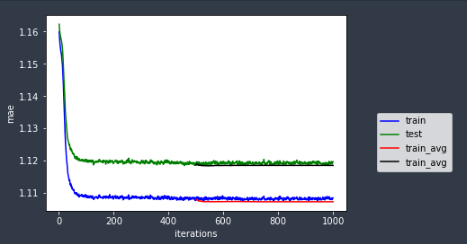
\includegraphics[scale=0.5]{mae_p2.png}
\caption{MAE vs Iterations (train\_avg and test\_avg are computed using Monte Carlo averaging)}
\label{mae}
\end{center}
\end{figure}

\begin{figure}[h!]
\begin{center}
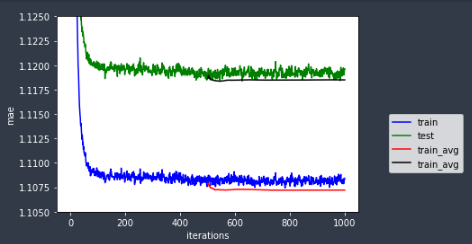
\includegraphics[scale=0.5]{mae_p2_zoom.png}
\caption{MAE vs Iterations (zoomed)}
\label{maeZ}
\end{center}
\end{figure}
\textit{Prominent Words for K topics} \\ \\

\begin{figure}[h!]
\begin{center}

\includegraphics[scale=0.45]{topics.png}
\caption{Prominent Words for each column of V (topics)}
\label{topics}
\end{center}
\end{figure}

There are multiple lists which seem to correspond to some "topic". For example, in Figure \ref{topics}, words for column 2 correspond to \emph{website extensions}. Similarly, words for column 3 correspond to \emph{science}, words for column 6 correspond to \emph{sports} etc. However, words for some columns like column 5 or 13 don't seem to correspond to a single topic. \\ \\
\emph{Columns clearly corresponding to a topic: } 2,3,6,7,12,14,16,17,20

\section*{Problem 3}
\textbf{Implementing MH Sampling for 2-D Gaussian} \\ \\
\emph{Code: mh\_sampling.py} \\ \\
Acceptance Rates for different values of variances are: \\
\emph{Variance = 0.01 : Acceptance = 0.92} \\
\emph{Variance = 1 : Acceptance = 0.40}\\
\emph{Variance = 100 : Acceptance = 0.01} \\ \\
Variance = 1, seems to be the best choice since it seems to produce good samples(Figure \ref{mh}) with satisfactory acceptance rate. Low Acceptance Rate implies more time for generating the same number of samples.

\begin{figure}[h!]
\begin{center}
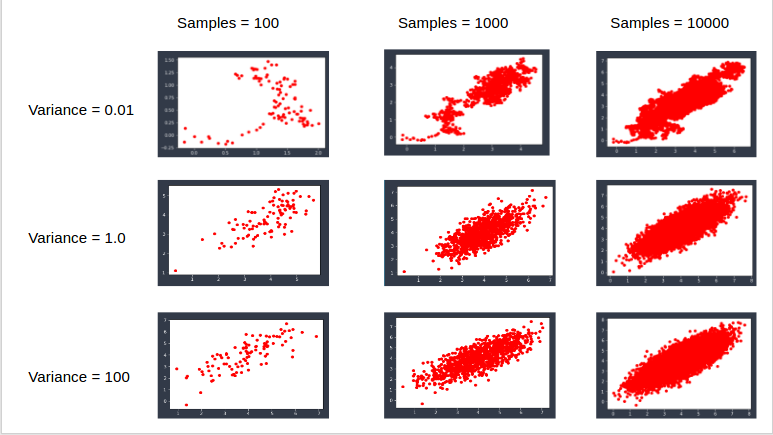
\includegraphics[scale=0.65]{plots_mh.png}
\caption{Plots for different variances and number of samples}
\label{mh}
\end{center}
\end{figure}



\section*{Problem 4}
\textbf{Mixture of Gaussians with Missing Data} \\ \\
As we know, the CLL for mixture of gaussians without missing data is given by:
$$\sum_{n=1}^N\sum_{k=1}^K z_{nk}[\log \pi_k + \log \mathcal{N}(x_n|\mu_k, \Sigma_k)]$$
In this problem with missing data, the expression for complete data log-likelihood(CLL) is given by:
$$\sum_{n=1}^N\sum_{k=1}^K z_{nk}[\log \pi_k + \log \mathcal{N}([x_n^{o}, x_n^{m}]|\mu_k, \Sigma_k)]$$
where $\pi_k$ is the mixing proportion for the $k^{th}$ cluster and $z_{nk}$ is 1 only when $n^{th}$ example belongs to the $k^{th}$ cluster, otherwise 0. $x_n^m$ and $x_n^o$ are the missing and observed parts of $x_n$ respectively. The expression for Expected CLL simplifies to:
$$\sum_{n=1}^N\sum_{k=1}^K \mathds{E}[z_{nk}][\log \pi_k - \frac{1}{2}\log |\Sigma_k| - \frac{1}{2}\text{trace}[\Sigma_k^{-1}\mathds{E}[S_k]]]$$
where $S_k$ is given by $(x_n-\mu_k)(x_n-\mu_k)^T$, because $x_n$ also contains $x_n^m$, which is missing(latent). Expectations required are:
\begin{itemize}
\item $\mathds{E}[z_{nk}]$ --  Computing this is similar to the regular GMM case and is given by:
$$\mathds{E}[z_{nk}] = \frac{\pi_k\mathcal{N}(x_n|\mu_k, \Sigma_k)}{\sum_{l=1}^K \pi_l\mathcal{N}(x_n|\mu_l, \Sigma_l)}$$
where $x_n = [x_n^m, x_n^o]$. Here, $x_n^m$ has to be replaced by $\mathds{E}[x_n^m]$, to be computed in next step. This can be initialized randomly for the first iteration.
\item $\mathds{E}[S_{k}]$ -- This can be computed in a similar manner as done in the midsem exam question. We only need to compute $\mathds{E}[x_n^m]$ and $\mathds{E}[x_n^mx_n^{mT}]$ for $\mathds{E}[S_{k}]$. The posterior $p(x_n^m|x_n^o, z_n=k)$, simplifies to:
$$p(x_n^m|x_n^o, \mu_k, \Sigma_k)$$
As we know, that $p(x_n^m|x_n^o, \mu_k, \Sigma_k)$ is a gaussian. $E[x_n^m]$ is then given by the mean of the gaussian $p(x_n^m|x_n^o, \mu_k, \Sigma_k)$. $\mathds{E}[x_n^mx_n^{mT}]$ can be computed as $\mathds{E}[x_n^m]\mathds{E}[x_n^{m}]^T + $ variance of the gaussian $p(x_n^m|x_n^o, \mu_k, \Sigma_k)$.
$$E[x_n^m] = \mu_{m} + \Sigma_{mo}\Sigma_{oo}^{-1}(x_n^o-\mu_o)$$
where $\mu_{m}$ and $\mu_{o}$ are the means of marginal gaussians which can be obtained by marginalising their joint pdf. The other symbols have their usual meaning. Also, the variance of the gaussian $p(x_n^m|x_n^o, \mu_k, \Sigma_k)$ is given by:
$$\Sigma_{mm}-\Sigma_{mo}\Sigma_{oo}^{-1}\Sigma_{om}$$
\end{itemize}

\emph{M Step} \\ \\
The updates are similar to the regular GMM case, the difference being that all the expressions like $x_n$ and $x_nx_n^T$ have to replaced by their expectations computed above. The final expressions for updates of $\{\pi_k, \mu_k, \Sigma_k\}_{k=1}^K$ are therefore :
$$\mu_k = \frac{1}{N_k}\sum_{n=1}^N \gamma_{nk}\mathds{E}[x_n]$$
$$\Sigma_k = \frac{1}{N_k}\sum_{n=1}^N \gamma_{nk}\mathds{E}[S_k] $$
$$\pi_k = \frac{N_k}{N}$$
where $N_k = \sum_{n=1}^N \gamma_{nk}$ and $\gamma_{nk}= \mathds{E}[z_{nk}]$. Also. $\mathds{E}[x_n]=[x_n^o, \mathds{E}[x_n^m]]$

\end{document}


